
\section{The Storybook}
The storybook contains all of the stories you can play in Wheel of Elements.
Each story will take about 2.5 hours to play through. One session includes 3 encounters and one text containing a short story for why you are fighting.

\begin{figure}[ht]
	\begin{minipage}[t][8cm][t]{0.5\textwidth}
		\begin{minipage}[t][5cm][t]{0.9\textwidth}
			\fbox{\parbox[4cm]{\textwidth}{Picture:  Merfolk storyteller teaching little frogs about the cosmic horrors}}
		\end{minipage}
	\end{minipage}
	\begin{minipage}[t][8cm][t]{0.5\textwidth}
		
		\subsection*{Stories}
		Each story begins with an introduction, which should be narrated by a player.
		The text is separated into four sections. After reading a section, start one of the three fights. After finishing a fight, read the next section, draw an event  \textit{See Page \pageref{Section_Events}} and level up \textit{See Page \pageref{Section_CharacterBuilding}}. Repeat this process after finishing the second encounter.
		%Flowchart? with nice pics?
		
		
		\subsection*{Encounters}
		Each story comes with three enemy encounters. An encounter presents which enemies should be fought and in which arrangement.
		There are always 5 enemy setups described per encounter. Each player takes one setup, matching the seating order.
		These enemy setups are distributed in clockwise seating order. %Please get  a picture for this
		If you are playing with less than 5 players, ignore the setups beyond your player number.
		After the first and second encounter, you level up. \textit{See Page \pageref{Section_CharacterBuilding}}
		
	\end{minipage}	
	
	%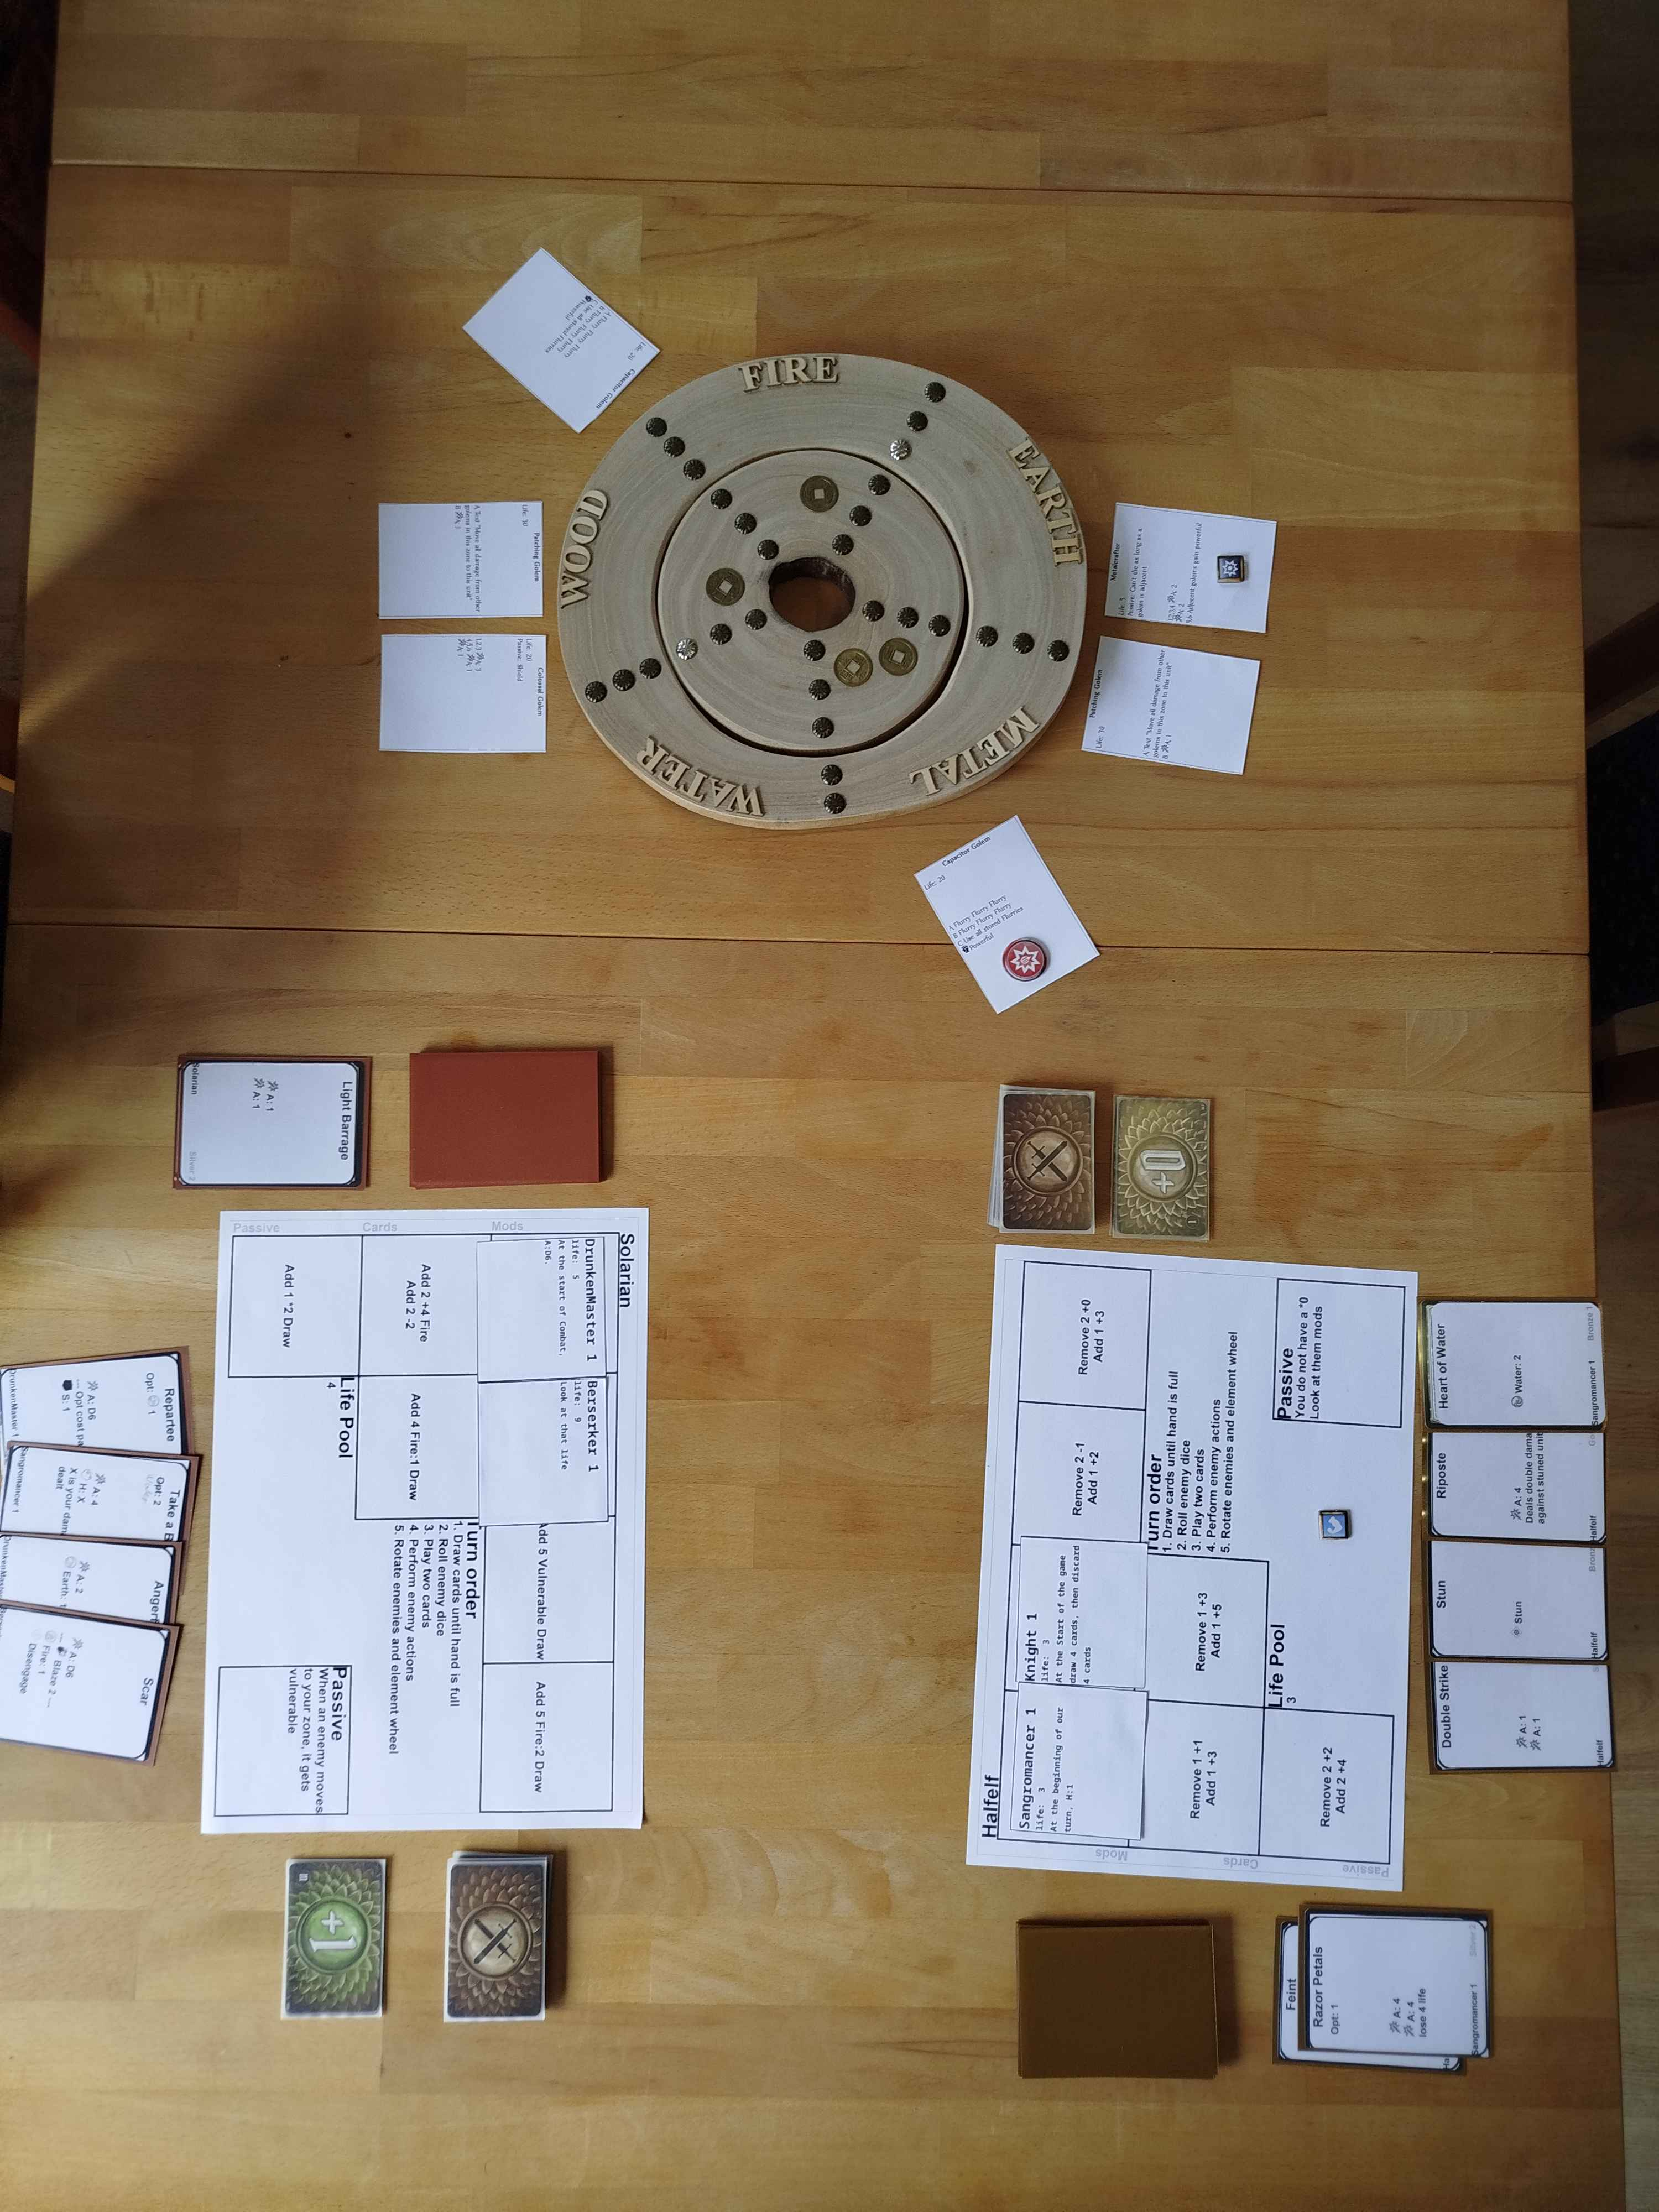
\includegraphics[width=0.8\textwidth]{ExplanationPics/TwoBoards.jpg}
\end{figure}


\section{Events}
\label{Section_Events}
\begin{figure}[ht]
	\begin{minipage}[t][6.5cm][t]{0.5\textwidth}
		Between two encounters (and before levelling up), you party will encounter events. These will change how you play the rest of the story. All events have an upside and a downside which will affect your choices and gameplay.
		Some events will make the game harder, and some easier. Some will warp your choices around them, and some may barely affect you. The only guarantee is that no two stories will play out the same.
	\end{minipage}	
	\begin{minipage}[t][6.5cm][t]{0.5\textwidth}
		\centering
		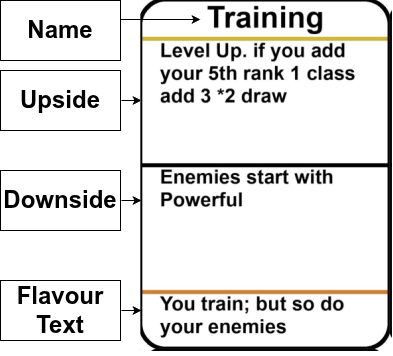
\includegraphics[width=0.9\linewidth, valign=t]{ExplanationPics/Event.drawio.png}
	\end{minipage}
\end{figure}
\begin{tcolorbox}[colframe=black, colback=white]
	Events happen before the level up, so consider adapting your future choices to the situation at hand.
\end{tcolorbox}

\fbox{\parbox[4cm]{\textwidth}{Picture:  Dragon flying overhead of some Solarians/Wyrmlings}}